\section{Standardisierung der Schnittstellennavigation} \label{sec:analyse-navigation}

Wie insbesondere bei ergonomischen Inspektionen und Benutzertests beobachtet wurde, kann die Schnittstelle für den Benutzer manchmal verwirrend sein, da er oft den roten Faden der Schnittstelle zu verlieren scheint.
Dennoch gibt es zahlreiche Regeln und Standards für Schnittstellen, die es dem Benutzer erleichtern, sich in einer komplexen Schnittstelle zurechtzufinden.
In diesem Abschnitt werden einige Strategien vorgestellt, die in der endgültigen Schnittstelle implementiert werden.

\subsection{Lokalisierung von Seiten}

Wenn ein Benutzer zwischen verschiedenen Seiten einer Webanwendung navigiert, muss er sehr schnell erkennen können, auf welcher Seite er sich befindet.
Wenn er keine normierte Referenz auf der Schnittstelle hat, kann es ihn Zeit und kognitive Belastung kosten, die Schnittstelle zu identifizieren, auf der er sich befindet, und die Verbindung nachzuvollziehen, die sie mit den anderen Schnittstellen der Anwendung hat.
Dies kann passieren, wenn sie viel zurückgehen, um eine zuvor geöffnete Seite erneut zu besuchen, oder wenn sie von einer Seite zu einer anderen weitergeleitet werden.
Schlimmer noch, wenn der Nutzer auf eine neue Seite gelangt, die er nicht kennt, muss er die Schnittstelle untersuchen, um zu versuchen, den Kontext der Seite zu erfassen, was eine unnötige Anstrengung erfordert.
Die beiden folgenden Beispielseiten haben zum Beispiel keine klaren Elemente, die es dem Nutzer ermöglichen, schnell zu erkennen, auf welcher Seite er sich befindet.

\begin{figure}[H]
  \centering
  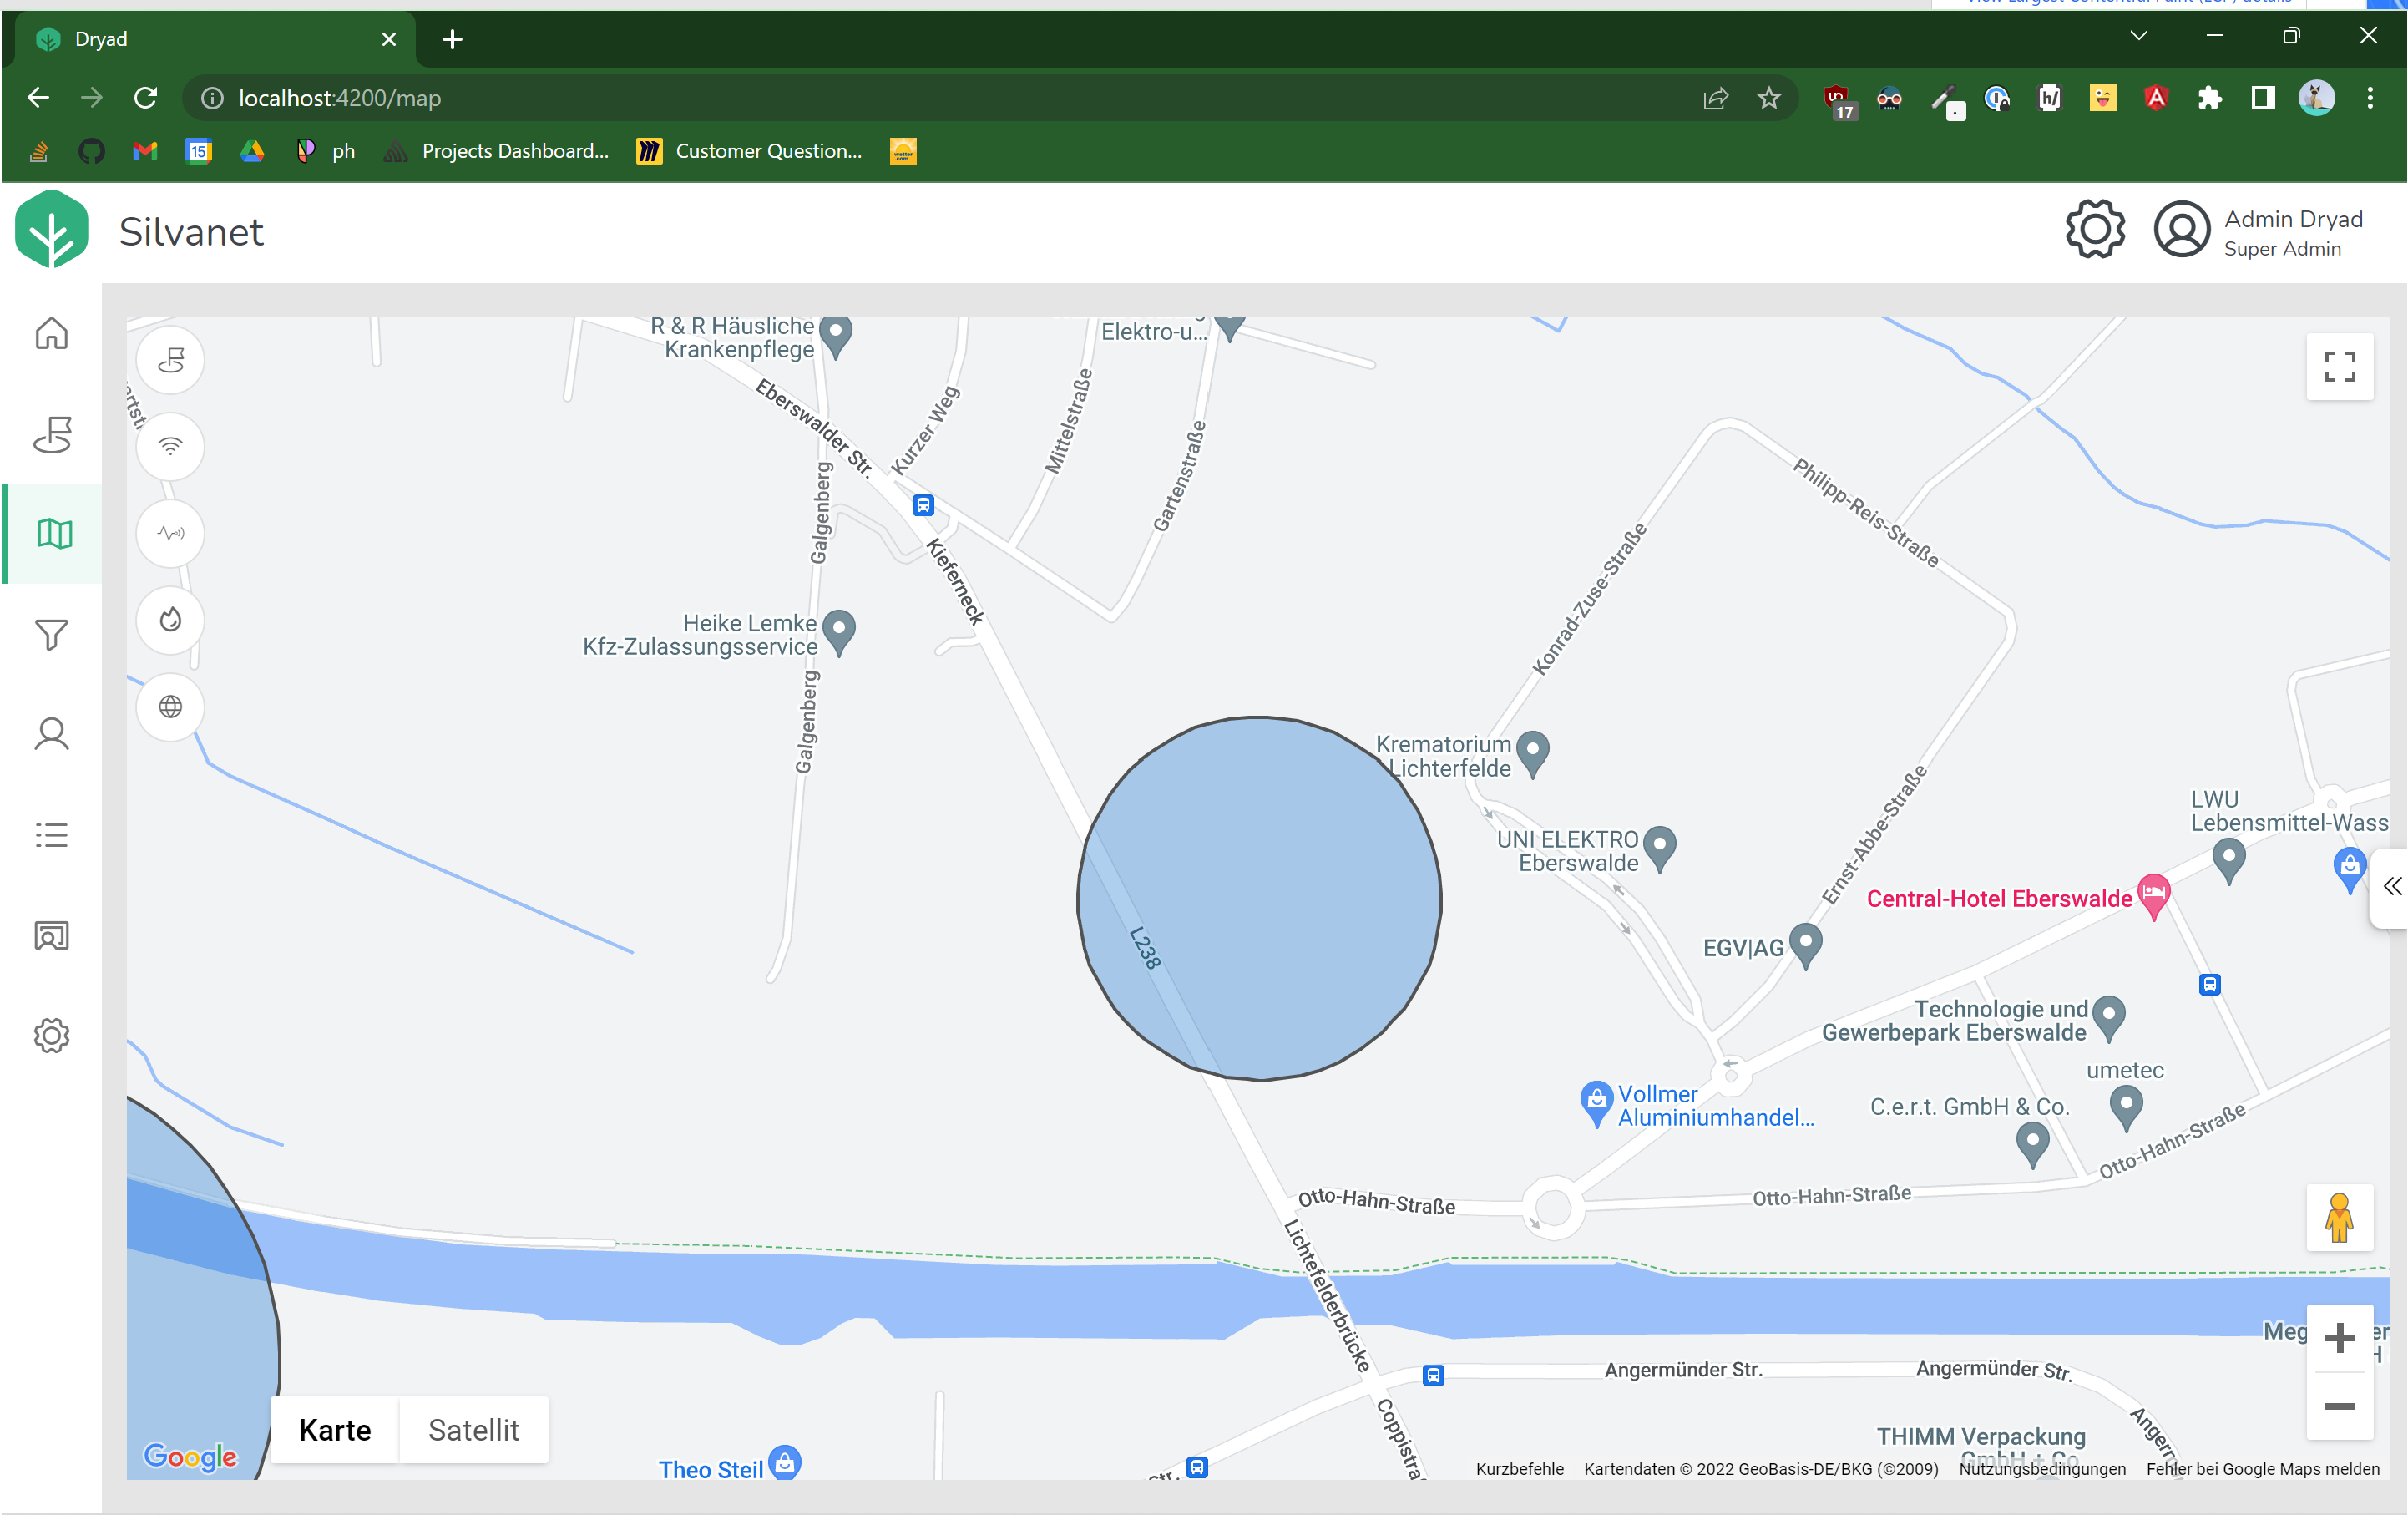
\includegraphics[width=\textwidth]{app_page_map_old}
  \caption{Seite der Schnittstelle mit einer interaktiven Karte der verschiedenen \textit{Sites}}
  \label{fig:app_page_map_old}
\end{figure}
\begin{figure}[H]
  \centering
  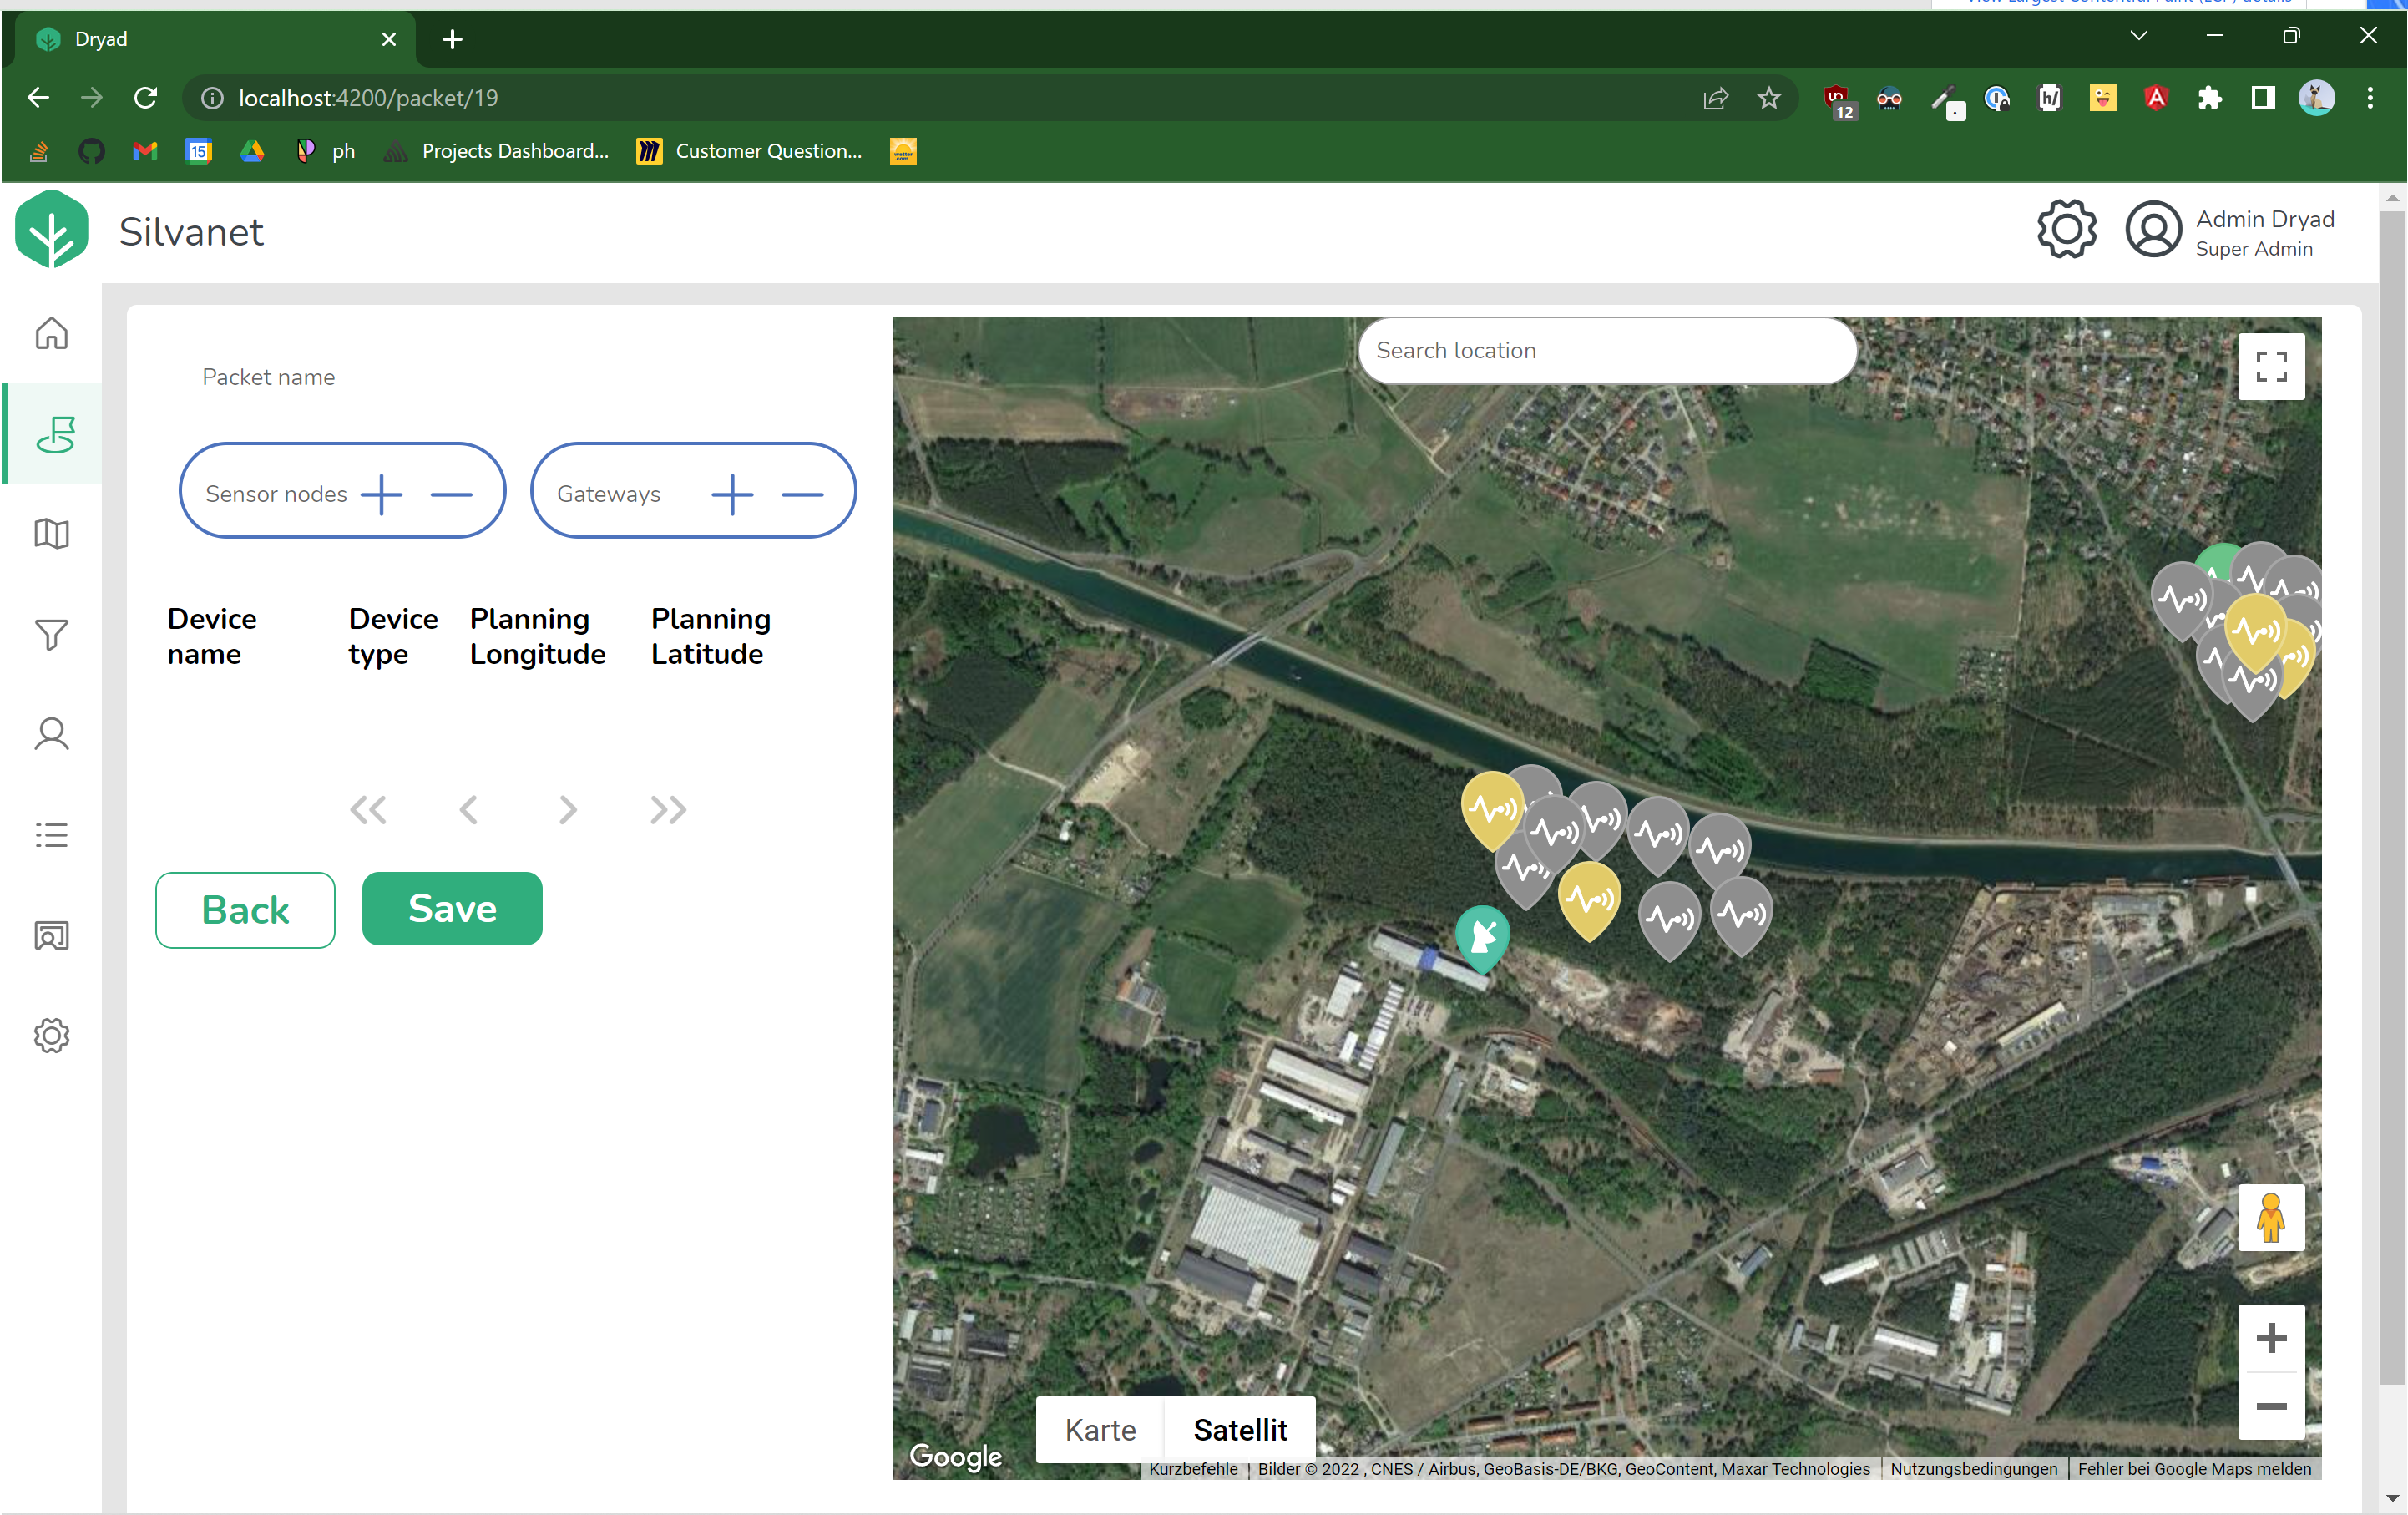
\includegraphics[width=\textwidth]{app_page_planning_old}
  \caption{Seite der Schnittstelle, mit der Sie den Einsatz von Sensoren an einem \textit{Sites} planen können.}
  \label{fig:app_page_planning_old}
\end{figure}

Auf diese Weise ist es für einen Nutzer nicht möglich, zu definieren, auf welcher Seite er sich befindet.
Es gibt jedoch viele standardisierte Strategien, die ein entspanntes Surfen ermöglichen.
Die erste, die sogar ein Muss für die Zugänglichkeit einer Schnittstelle ist, ist das Vorhandensein eines aussagekräftigen Seitentitels.
Dieser Seitentitel wird in \ac{HTML} im Header der Seitenstruktur deklariert und ermöglicht es, einen benutzerdefinierten String in der Titelleiste des Browsers, im Seitenfenster oder auch im Verlauf des Browsers anzuzeigen.
Anhand eines aussagekräftigen Titels kann ein Benutzer leicht erkennen, welche Webseite er gerade benutzt und wann sich die Webseite geändert hat.
Der Titel kann zur Identifizierung der Webseite verwendet werden, ohne dass die Benutzer den Inhalt der Seite lesen oder interpretieren müssen.
Die Benutzer können den gewünschten Inhalt schneller finden, wenn genaue, beschreibende Titel in Sitemaps oder Listen von Suchergebnissen erscheinen.

So empfehlen die Zugänglichkeitsstandards der \ac{WCAG}\cite{wcag}, dass der Titel einer Seite in der Lage ist:

\begin{itemize}
  \item Das Thema der Webseite identifizieren
  \item Sinn machen, wenn sie ohne Kontext gelesen werden, z. B. in einer Website-Karte oder einer Liste von Suchergebnissen
  \item Kurz sein
  \item Angabe der Website oder einer anderen Ressource, zu der die Webseite gehört
\end{itemize}

Eine Struktur, die von der großen Mehrheit der Web-Schnittstellen verwendet wird, kann durch die folgende Notation dargestellt werden\\
\lstinline{<Eindeutiger Titel der Seite> <Trenner> <Titel der Anwendung>}.

Im Fall der Silvanet-Anwendung von Dryad wurden die folgenden Standards festgelegt:

\begin{itemize}
  \item \textbf{<Titel der Anwendung>}: Dryad
  \item \textbf{<Trenner>}: •
\end{itemize}

Die Anwendung muss also in der Lage sein, für jede Seite einen Titel vorzuschlagen, der diesem Standard entspricht.
Jetzt müssen Sie dem Nutzer auch noch einen Seitentitel anbieten, der für die Seite selbst relevant ist.
Wie man in \ref{fig:app_page_map_old} und \ref{fig:app_page_planning_old} sehen kann, bleibt der Haupttitel der Seite, der dem \lstinline{h1}-Tag in \ac{HTML} entspricht, nämlich konstant das gleiche Wort \textit{Silvanet}.

Die Schnittstelle sollte an dieser Stelle auch einen Begriff verwenden, der den Kontext der Seite beschreibt, so dass er den Seitentitel widerspiegelt.
Hier ist ein Beispiel für eine Kombination von Seitentiteln mit einem relevanten, standardisierten und kontextbezogenen Hauptseitentitel.

\begin{table}[H]
  \begin{tabular}{p{0.5\linewidth} |p{0.5\linewidth}}
    Seitentiteln                   & Hauptseitentitel \\ \hline\hline

    \textit{Sites • Dryad}         & Sites Management \\\hline
    \textit{User Settings • Dryad} & User Settings    \\\hline
    \textit{Dashboard • Dryad}     & Dashboard
    \\\hline
  \end{tabular}
  \caption{Beispiel für eine Kombination von Seitentiteln mit einem Hauptseitentitel}
\end{table}

\subsection{Übersichtliches Navigationssystem}

Die Navigation des Nutzers sollte so einfach wie möglich gestaltet werden, damit es keine Ambiguität gibt, die es dem Nutzer erlaubt, die Oberfläche selbst zu erkunden.
Die ergonomische Inspektion \ref{appendix:ergonomic-inspection} zeigt jedoch einen großen Usability-Fehler in der Seitenleiste der Anwendung, die als Navigationsmenü fungiert.
Es besteht nur aus Icons, die, wie im Punkt \ref{sec:guidance} erläutert, sehr subjektiv und hängen von der Kultur des Nutzers ab.
Es ist daher notwendig, jedem Icon ein Textlabel hinzuzufügen, um die Verständlichkeit der Icons im Menü zu standardisieren.
Dies nimmt jedoch Platz auf der Benutzeroberfläche in Anspruch, da der Benutzer diese Aktion schnell beherrschen und verstehen muss.
Nach mehreren Besuchen auf der Benutzeroberfläche wird der Benutzer natürlich eine Verbindung zwischen den Icons und dem Label herstellen.
So ist es sinnvoll, dass der Nutzer jederzeit entscheiden kann, ob er die Textkennzeichnungen ausblenden oder anzeigen möchte.
In dieser Situation kann ein Kollaps-System verwendet werden.

\begin{table}[H]
  \begin{tabular}{p{0.5\linewidth} |p{0.5\linewidth}}
    Menü mit Textlabels & Reduziertes Menü nur mit Icons \\ \hline\hline

    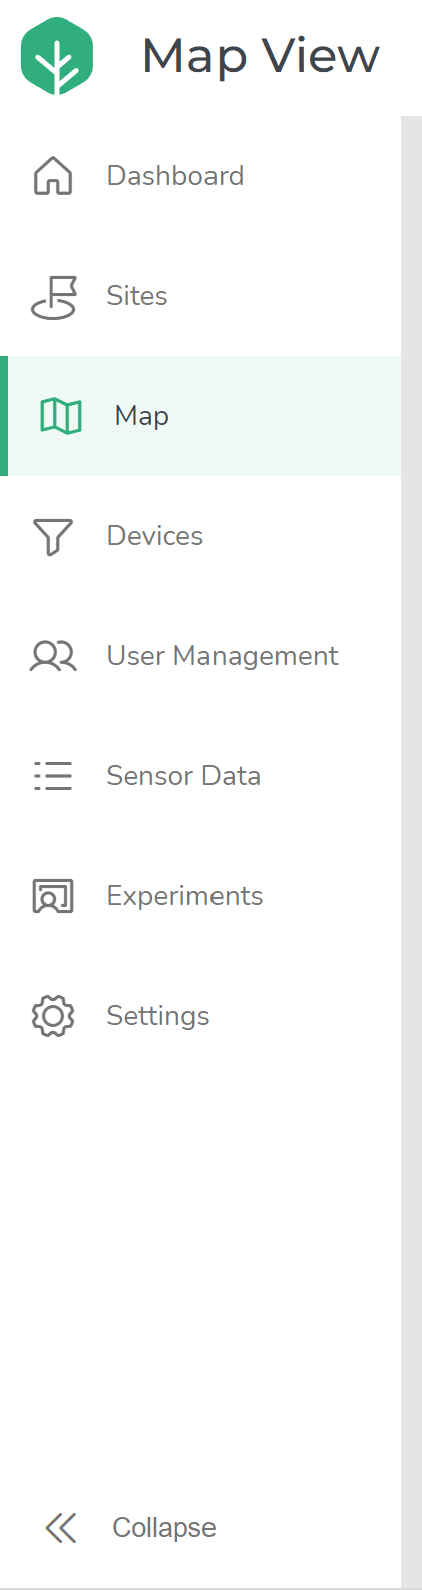
\includegraphics[height=12cm]{app_sidebar_open}
                        &
    
\includegraphics[height=12cm]{app_sidebar_collapsed}
  \end{tabular}
  \caption{Menü in der Sidebar, das ein Kollaps-Design implementiert}
\end{table}

Ein weiterer nicht zu vernachlässigender Aspekt der Schnittstelle bleibt, dem Benutzer zu zeigen, wo er sich in der Hierarchie der Anwendung befindet.
Ein UI-Element, das so alt ist wie das Web selbst, ist immer noch führend in diesem Bereich, da es dem Nutzer ermöglicht, mit einem Klick auf die oberen Ebenen der Website zu gelangen, wenig Platz auf der Benutzeroberfläche einnimmt und als sekundäres Navigationsmittel dient: die Breadcrumb \cite{breadcrumb}.
Breadcrumbs sind eine Liste von Links, die die aktuelle Seite und ihre "Vorgänger" (übergeordnete Seite, Großelternseite usw.) darstellen und in der Regel bis zur Startseite der Website zurückreichen.

\begin{figure}[H]
  \centering
  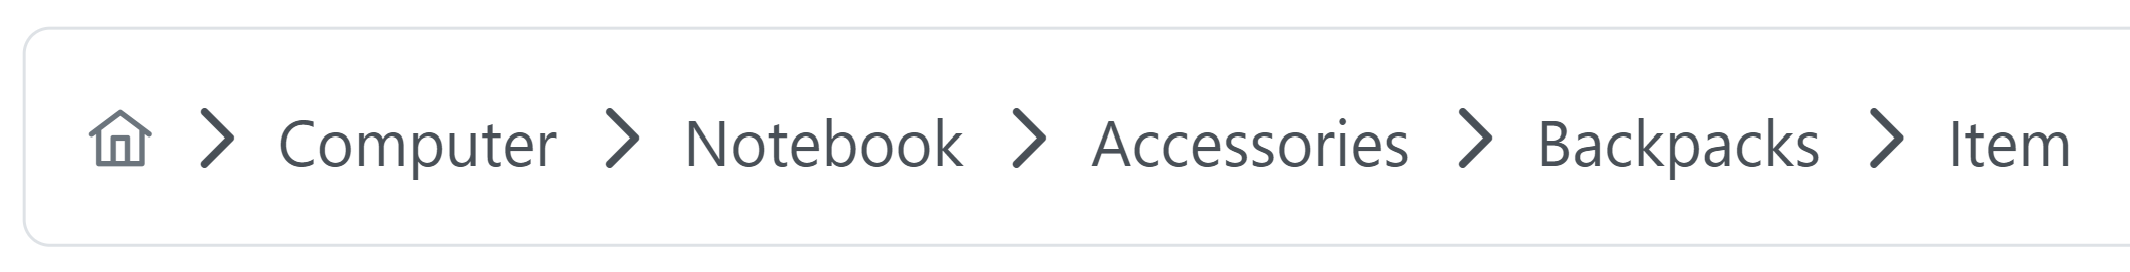
\includegraphics[width=12cm]{primeng_breadcrumb}
  \caption{Beispiel einer breadcrumb-Komponente, die von der PrimeNg-Bibliothek \ref{sec:primeng} gerendert wurde}
  \label{fig:primeng_breadcrumb}
\end{figure}

Die Schnittstelle muss eine generische Logik implementieren, die es ermöglicht, dem Benutzer auf jeder verfügbaren Seite eine Breadcrumb-Komponente anzuzeigen.
Diese muss so gestaltet sein, dass das Hinzufügen von Seiten nicht dazu führt, dass der Code, der mit der Breadcrumb-Komponente verknüpft ist, in irgendeiner Weise manipuliert werden muss.

\subsection{Hierarchie der Anwendung}

Mit der breadcrumb-Komponente können Sie die Tiefenstruktur einer Seite anzeigen.
Allerdings muss die Anwendung als Ganzes eine Tiefenstruktur aufweisen, damit Sie Seiten leicht in Gruppen zusammenfassen können.
Wenn man sich die Sitemap ansieht, erkennt man eine sehr flache Hierarchie, die die Navigation auf der Seite sehr kompliziert macht.

\begin{figure}[H]
  \centering
  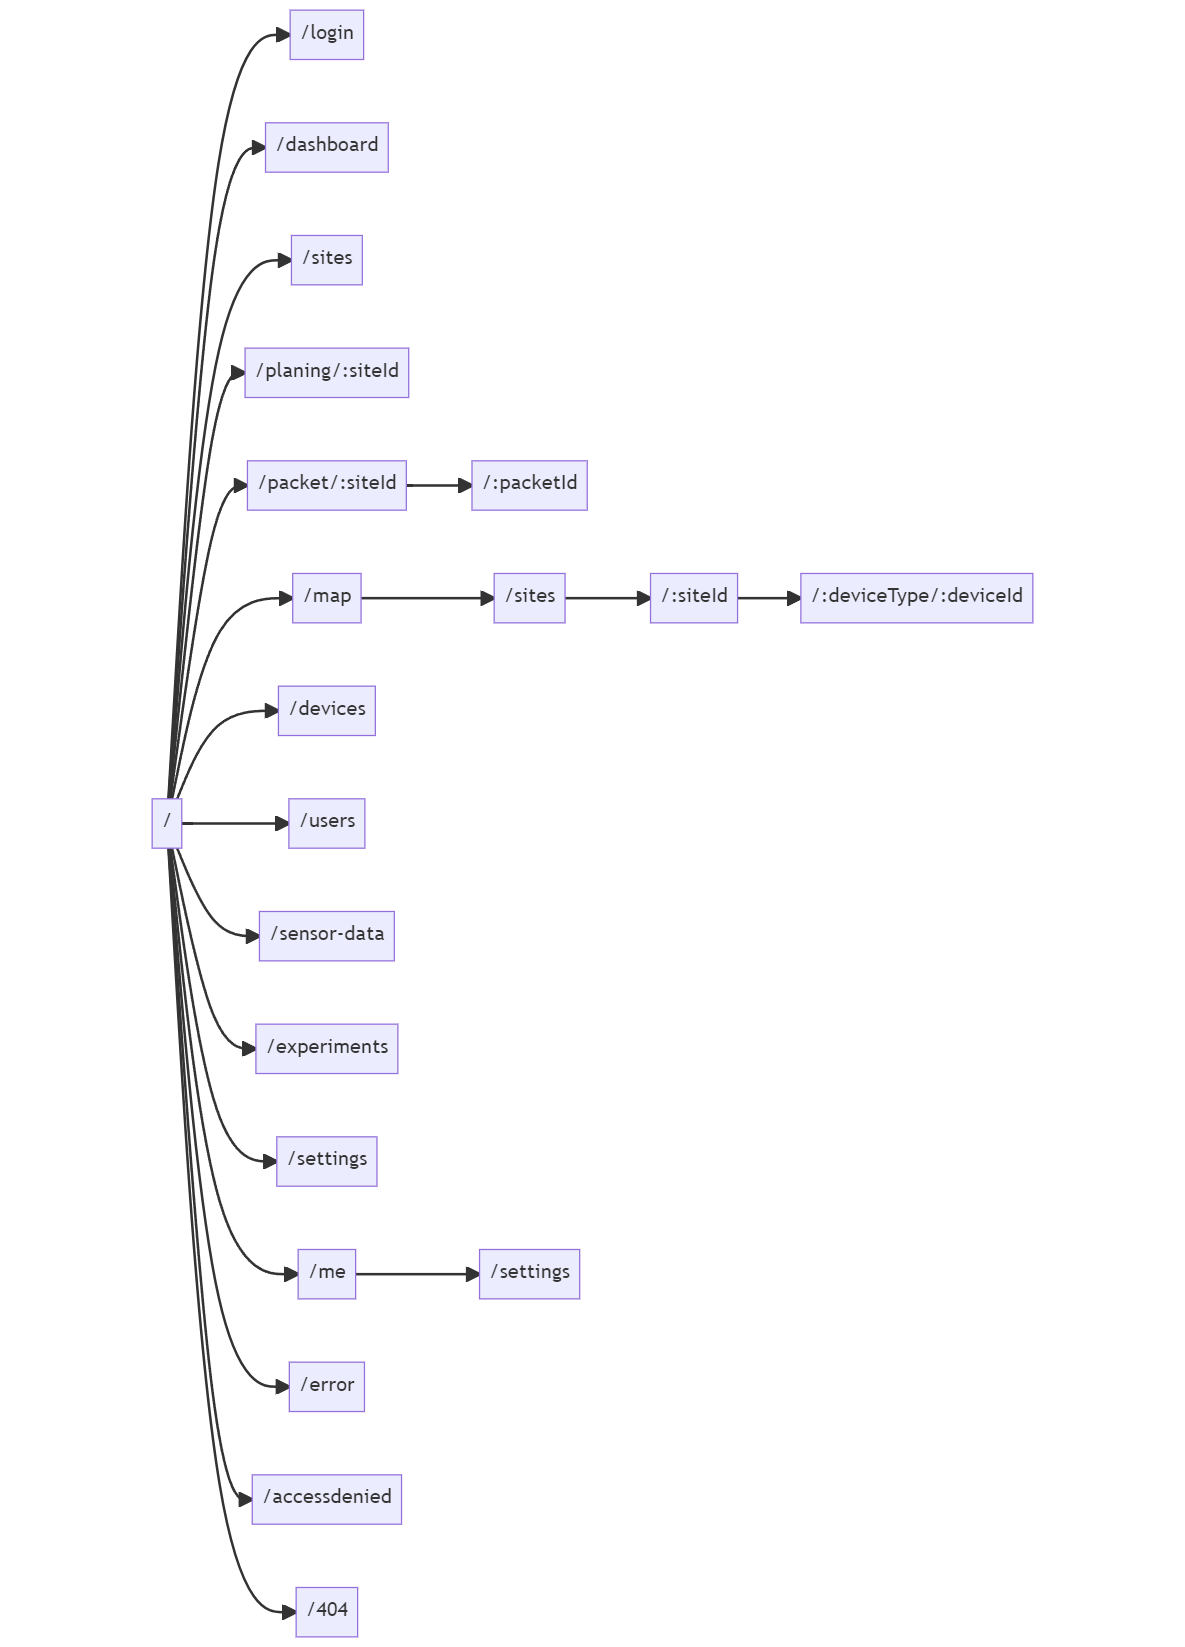
\includegraphics[width=12cm]{site_map}
  \caption{Schematische Darstellung der Sitemap, die alle zugänglichen Seiten und ihre Vorgänger zeigt}
  \label{fig:site_map}
\end{figure}

Das Routing der Dryad-Anwendung muss daher neu bewertet werden, um eine Downlink-Architektur zu bieten.
Ein sinnvoller Ansatz für diese Aufgabe ist es, sich auf eine starke URL-Hierarchie-Konvention wie das berühmte \ac{REST} zu stützen.

\subsubsection{REST-Konvention der URIs}

Die REST-Konvention ermöglicht eine primäre und standardisierte Darstellung der verschiedenen Daten, die als Ressource bezeichnet werden.
Die Einführung einer einheitlichen und robusten Strategie zur Benennung von REST-Ressourcen wird sich als eine der besten langfristigen Designentscheidungen erweisen.
In REST kann eine Ressource das sein, was als Singleton oder Sammlung bezeichnet wird.
Zum Beispiel ist die Ressource \lstinline{users} eine Sammlung und die Ressource \lstinline{user} ist ein Singleton.
In diesem Fall kann auf die Sammlung mit dem \ac{URI} \lstinline{/users} und auf das Singleton anhand seiner Kennung mit dem \ac{URI} \lstinline{/users/:userId} zugegriffen werden.
Dies gilt in gleicher Weise für Untersammlungen wie z. B. ein Singleton \lstinline{article} eines \lstinline{user}.
Dieser wird über \lstinline{/users/:userId/articles/:articleId} erreichbar, wobei das Zeichen \lstinline{/} eine hierarchische Beziehung anzeigt.

Die REST-Konvention legt außerdem die folgenden Regeln fest:

\begin{itemize}
  \item Der Name einer Ressource muss immer im Plural stehen.
  \item Wenn der Name einer Sammlung aus mehreren Wörtern besteht, müssen diese durch einen Bindestrich getrennt werden.
  \item Der \ac{URI} muss in Kleinbuchstaben definiert werden.
\end{itemize}

\subsubsection{Anwenden der REST-Konvention auf die Anwendung}

In der vorliegenden Form ermöglicht es die REST-Konvention praktisch, das Routing aller unserer Seiten auf strukturierte Weise zu erstellen.
Dies ist der Fall bei Seiten, die eine Sammlung oder ein Singleton anzeigen wollen, aber bei sogenannten Aktionsseiten muss noch einiges getan werden.
In der reinen REST-Konvention werden Aktionen direkt durch die \ac{HTTP}-Verben POST, DELETE, PUT definiert, da die Konvention mit dem Ziel entwickelt wurde, Webdienste über \ac{HTTP} zu erstellen.
Diese Verben sind für das Routing einer Webanwendung nicht verwendbar, also muss eine Alternative gefunden werden.
Die Strategie besteht darin, diese Verben einfach auszudrücken, indem man einen URI an den URI der betreffenden Ressource oder des betreffenden Singletons anhängt.
Dieser \ac{URI} wird ein englisches Wort sein, das die Aktion so präzisiert, dass ein Nutzer sie verstehen kann.
Um Aktions-\ac{URI}s von Ressourcen oder Singletons zu unterscheiden, wird ihnen ein Underscore vorangestellt.
Die Seite, auf der Sie einen neuen Benutzer anlegen können, hat z. B. den \ac{URI} \lstinline{/users/_create}.

\begin{table}[H]
  \begin{tabular}{p{0.5\linewidth} |p{0.5\linewidth}}
    HTTP-Verben     & Entsprechender URI               \\ \hline\hline

    \textbf{POST}   & \textbf{/\textunderscore create} \\\hline
    \textbf{PUT}    & \textbf{/\textunderscore edit}   \\\hline
    \textbf{DELETE} & \textbf{/\textunderscore delete}
  \end{tabular}
  \caption{Anpassung der \ac{HTTP}-Verben der \ac{REST}-Konvention für die Verwendung im Routing der Schnittstelle}
\end{table}

Mit der Umsetzung all dieser Regeln ist es schließlich möglich, eine standardisierte Architektur der Anwendung zu definieren:

\begin{figure}[H]
  \centering
  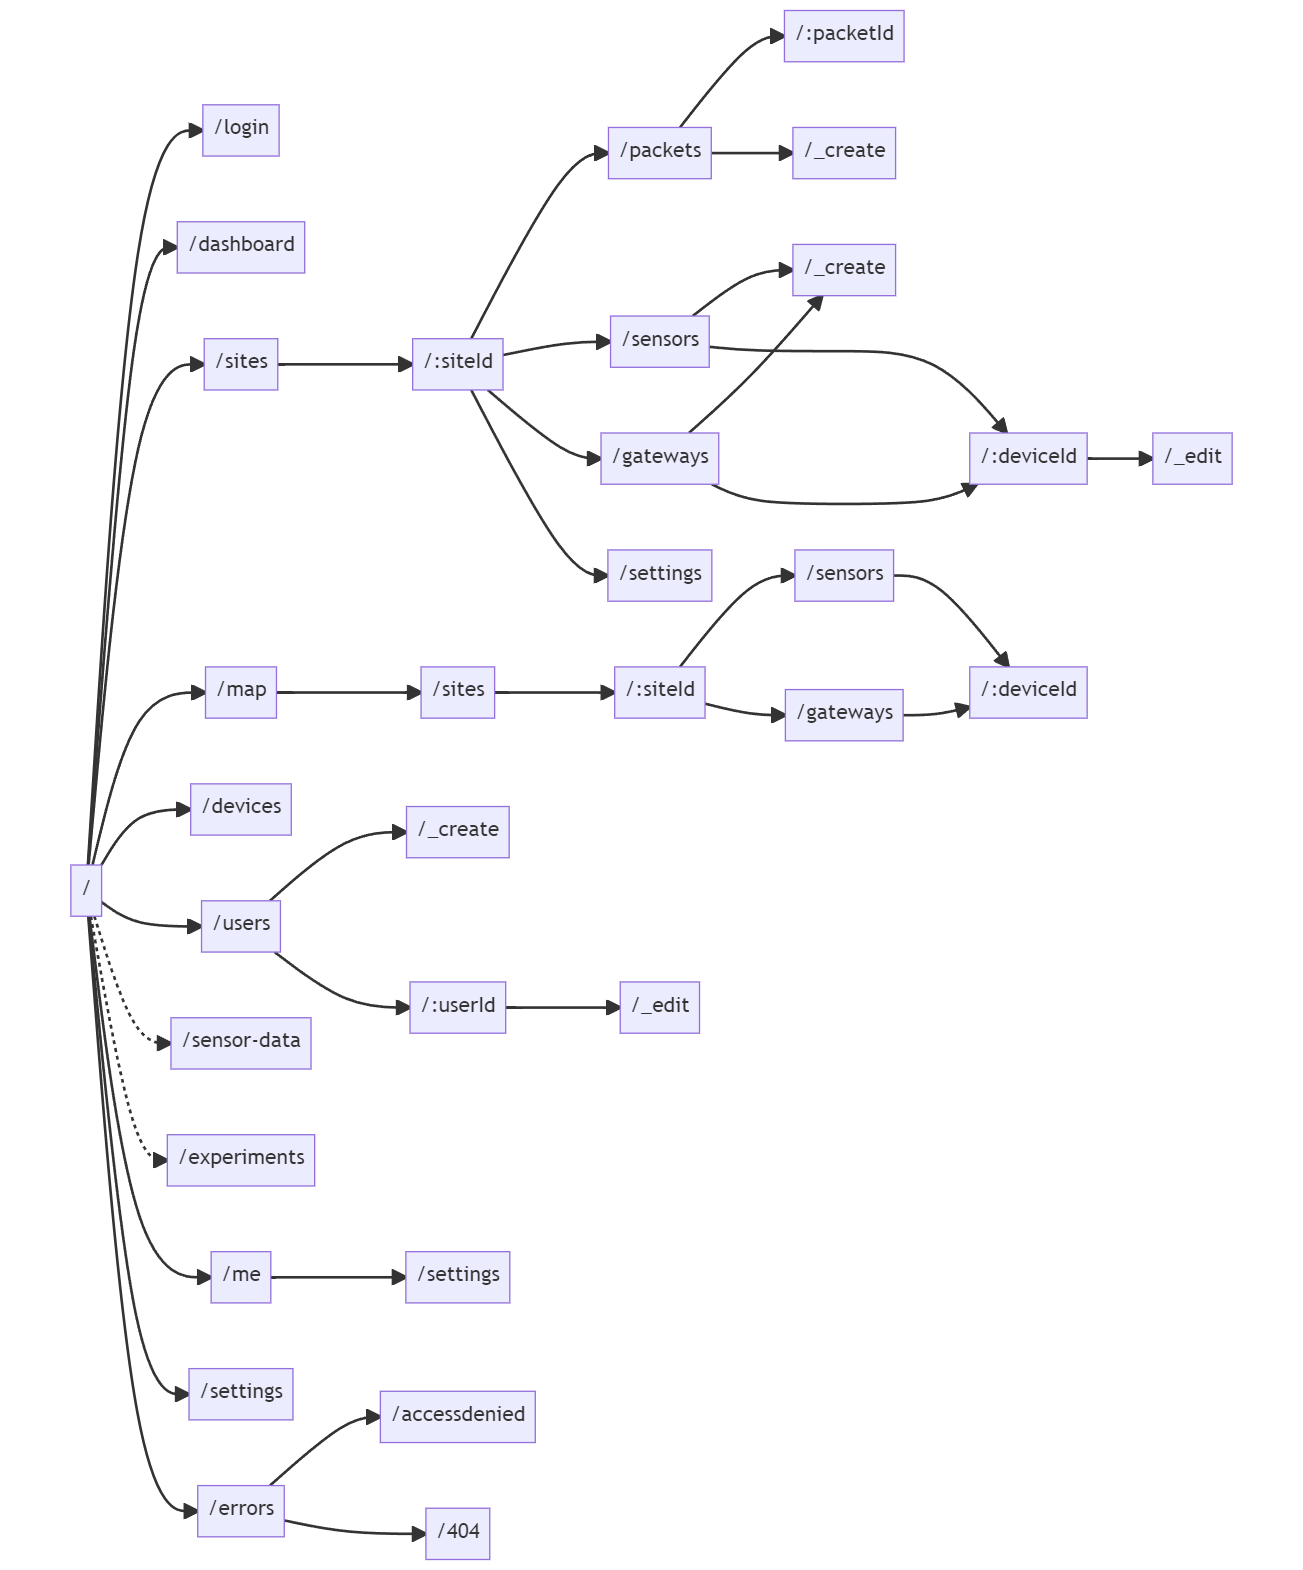
\includegraphics[width=\textwidth]{site_map_v2}
  \caption{Schematische Darstellung der Sitemap nach einer Normalisierung mit der angepassten Konvention von \ac{REST}}
  \label{fig:site_map_v2}
\end{figure}

So kann man direkt die Relevanz dieser Normierung erkennen, die es ermöglicht, eine flache Hierarchie in eine tiefere und organisiertere Baumstruktur zu verwandeln.
Dies hat auch den Vorteil, dass der Nutzer ganz einfach ganz bestimmte Seiten der Anwendung teilen kann.
Es würde zu lange dauern, die gesamte Hierarchie der aktuellen Anwendung zu refaktorisieren, daher wird sich die Thesis nur mit der Sammlung \lstinline{/sites} und ihren Nachkommen beschäftigen.
